\documentclass[14pt]{extbook}
\usepackage{multicol, enumerate, enumitem, hyperref, color, soul, setspace, parskip, fancyhdr} %General Packages
\usepackage{amssymb, amsthm, amsmath, latexsym, units, mathtools} %Math Packages
\everymath{\displaystyle} %All math in Display Style
% Packages with additional options
\usepackage[headsep=0.5cm,headheight=12pt, left=1 in,right= 1 in,top= 1 in,bottom= 1 in]{geometry}
\usepackage[usenames,dvipsnames]{xcolor}
\usepackage{dashrule}  % Package to use the command below to create lines between items
\newcommand{\litem}[1]{\item#1\hspace*{-1cm}\rule{\textwidth}{0.4pt}}
\pagestyle{fancy}
\lhead{Progress Quiz 3}
\chead{}
\rhead{Version B}
\lfoot{3012-8528}
\cfoot{}
\rfoot{Summer C 2021}
\begin{document}

\begin{enumerate}
\litem{
Find the equation of the line described below. Write the linear equation in the form $ y=mx+b $ and choose the intervals that contain $m$ and $b$.\[ \text{Parallel to } 4 x + 7 y = 6 \text{ and passing through the point } (-10, 7). \]\begin{enumerate}[label=\Alph*.]
\item \( m \in [0.13, 0.63] \hspace*{3mm} b \in [10.9, 13.8] \)
\item \( m \in [-1.26, -0.23] \hspace*{3mm} b \in [15.6, 17.4] \)
\item \( m \in [-1.26, -0.23] \hspace*{3mm} b \in [-1.4, -0.3] \)
\item \( m \in [-1.26, -0.23] \hspace*{3mm} b \in [1, 2.5] \)
\item \( m \in [-1.86, -1.45] \hspace*{3mm} b \in [1, 2.5] \)

\end{enumerate} }
\litem{
Solve the equation below. Then, choose the interval that contains the solution.\[ -2(18x + 15) = -17(5x + 4) \]\begin{enumerate}[label=\Alph*.]
\item \( x \in [-0.8, -0.75] \)
\item \( x \in [-2.07, -1.94] \)
\item \( x \in [-0.85, -0.8] \)
\item \( x \in [1.97, 2.04] \)
\item \( \text{There are no real solutions.} \)

\end{enumerate} }
\litem{
Write the equation of the line in the graph below in Standard Form $Ax+By=C$. Then, choose the intervals that contain $A, B, \text{ and } C$.
\begin{center}
    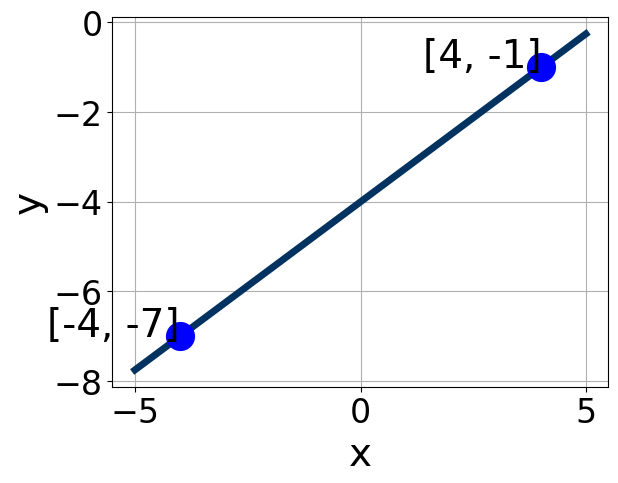
\includegraphics[width=0.5\textwidth]{../Figures/linearGraphToStandardCopyB.png}
\end{center}
\begin{enumerate}[label=\Alph*.]
\item \( A \in [0, 11], \hspace{3mm} B \in [-4.9, -2.1], \text{ and } \hspace{3mm} C \in [11, 17] \)
\item \( A \in [-5, -2], \hspace{3mm} B \in [3, 5.3], \text{ and } \hspace{3mm} C \in [-17, -13] \)
\item \( A \in [0, 11], \hspace{3mm} B \in [3, 5.3], \text{ and } \hspace{3mm} C \in [-17, -13] \)
\item \( A \in [-1.75, 1.25], \hspace{3mm} B \in [-1.9, -0.3], \text{ and } \hspace{3mm} C \in [4, 9] \)
\item \( A \in [-1.75, 1.25], \hspace{3mm} B \in [-0.9, 3.9], \text{ and } \hspace{3mm} C \in [-6, -3] \)

\end{enumerate} }
\litem{
Find the equation of the line described below. Write the linear equation in the form $ y=mx+b $ and choose the intervals that contain $m$ and $b$.\[ \text{Perpendicular to } 8 x - 7 y = 15 \text{ and passing through the point } (-8, 2). \]\begin{enumerate}[label=\Alph*.]
\item \( m \in [-0.95, -0.63] \hspace*{3mm} b \in [9.4, 12.2] \)
\item \( m \in [-0.95, -0.63] \hspace*{3mm} b \in [4.8, 7.4] \)
\item \( m \in [-0.95, -0.63] \hspace*{3mm} b \in [-5.7, -4.2] \)
\item \( m \in [-1.29, -0.91] \hspace*{3mm} b \in [-5.7, -4.2] \)
\item \( m \in [0.67, 0.93] \hspace*{3mm} b \in [8.9, 9.9] \)

\end{enumerate} }
\litem{
Write the equation of the line in the graph below in Standard Form $Ax+By=C$. Then, choose the intervals that contain $A, B, \text{ and } C$.
\begin{center}
    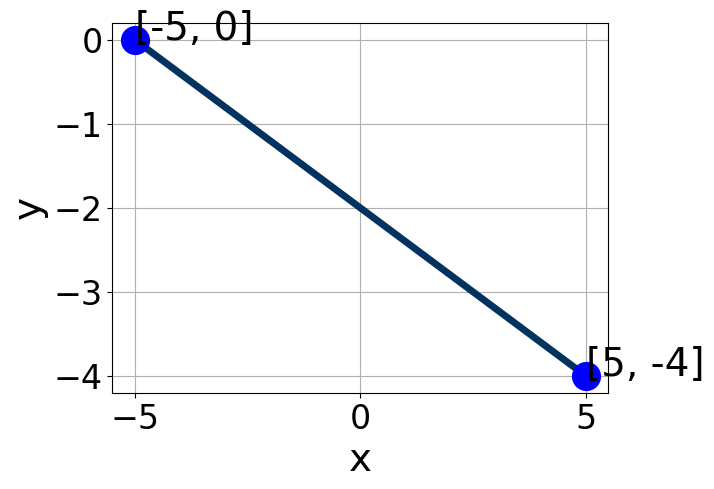
\includegraphics[width=0.5\textwidth]{../Figures/linearGraphToStandardB.png}
\end{center}
\begin{enumerate}[label=\Alph*.]
\item \( A \in [-0.74, 0.63], \hspace{3mm} B \in [-0.1, 3.7], \text{ and } \hspace{3mm} C \in [-3, 0] \)
\item \( A \in [-3.35, -0.07], \hspace{3mm} B \in [-8, -2.4], \text{ and } \hspace{3mm} C \in [10, 15] \)
\item \( A \in [0.71, 2.16], \hspace{3mm} B \in [3.6, 6.3], \text{ and } \hspace{3mm} C \in [-16, -9] \)
\item \( A \in [0.71, 2.16], \hspace{3mm} B \in [-8, -2.4], \text{ and } \hspace{3mm} C \in [10, 15] \)
\item \( A \in [-0.74, 0.63], \hspace{3mm} B \in [-2.5, 0.2], \text{ and } \hspace{3mm} C \in [1, 9] \)

\end{enumerate} }
\litem{
Solve the linear equation below. Then, choose the interval that contains the solution.\[ \frac{4x + 7}{8} - \frac{-5x -7}{4} = \frac{8x -5}{2} \]\begin{enumerate}[label=\Alph*.]
\item \( x \in [-8.12, -2.12] \)
\item \( x \in [7.44, 11.44] \)
\item \( x \in [-1.28, 1.72] \)
\item \( x \in [1.28, 4.28] \)
\item \( \text{There are no real solutions.} \)

\end{enumerate} }
\litem{
First, find the equation of the line containing the two points below. Then, write the equation in the form $ y=mx+b $ and choose the intervals that contain $m$ and $b$.\[ (5, -11) \text{ and } (-5, 4) \]\begin{enumerate}[label=\Alph*.]
\item \( m \in [0.8, 4.6] \hspace*{3mm} b \in [10.5, 16.5] \)
\item \( m \in [-2.8, -1.2] \hspace*{3mm} b \in [-22, -14] \)
\item \( m \in [-2.8, -1.2] \hspace*{3mm} b \in [5, 11] \)
\item \( m \in [-2.8, -1.2] \hspace*{3mm} b \in [-3.5, -0.5] \)
\item \( m \in [-2.8, -1.2] \hspace*{3mm} b \in [1.5, 8.5] \)

\end{enumerate} }
\litem{
Solve the linear equation below. Then, choose the interval that contains the solution.\[ \frac{5x + 4}{2} - \frac{3x -7}{8} = \frac{3x -6}{4} \]\begin{enumerate}[label=\Alph*.]
\item \( x \in [-3.7, -2.4] \)
\item \( x \in [3.3, 4.5] \)
\item \( x \in [-14.5, -11.3] \)
\item \( x \in [-2.2, -1.2] \)
\item \( \text{There are no real solutions.} \)

\end{enumerate} }
\litem{
Solve the equation below. Then, choose the interval that contains the solution.\[ -8(6x + 5) = -13(-4x + 7) \]\begin{enumerate}[label=\Alph*.]
\item \( x \in [32.18, 33.29] \)
\item \( x \in [-0.06, 0.79] \)
\item \( x \in [0.69, 2.49] \)
\item \( x \in [-1.35, -0.65] \)
\item \( \text{There are no real solutions.} \)

\end{enumerate} }
\litem{
First, find the equation of the line containing the two points below. Then, write the equation in the form $ y=mx+b $ and choose the intervals that contain $m$ and $b$.\[ (7, -11) \text{ and } (-7, -10) \]\begin{enumerate}[label=\Alph*.]
\item \( m \in [-0.11, -0.06] \hspace*{3mm} b \in [9.03, 10.59] \)
\item \( m \in [-0.11, -0.06] \hspace*{3mm} b \in [-11.27, -10.49] \)
\item \( m \in [-0.11, -0.06] \hspace*{3mm} b \in [-4.6, -1.23] \)
\item \( m \in [-0.11, -0.06] \hspace*{3mm} b \in [-18.5, -16.95] \)
\item \( m \in [0.04, 0.16] \hspace*{3mm} b \in [-9.63, -9.42] \)

\end{enumerate} }
\end{enumerate}

\end{document}